% !TeX root=../main.tex

\chapter{اتصال گره سبک به شبکهٔ همتابه‌همتای بیت‌کوین}
\label{app:p2p}
%\thispagestyle{empty}
در این پیوست نحوهٔ اتصال یک گره سبک به شبکهٔ همتا‌به‌همتای بیت‌کوین توضیح داده می‌شود. تمام  ارتباطات همتا‌به‌همتا در بیت‌کوین در بستر TCP برقرار می‌شود و تمام پیام‌ها از قالب یکسانی پیروی می‌کنند. رشتهٔ آغازین پیام‌ها و مقدار پیش‌فرض شمارهٔ درگاه با توجه به اینکه پیام در شبکهٔ اصلی، تست یا در حالت تست رگرسیون استفاده می‌شود تفاوت می‌کند. جدول \ref{table:PortandString} این مقادیر را نشان می‌دهد. یک گره می‌تواند از شمارهٔ درگاهی متفاوت در یک شبکه استفاده نماید.



\begin{xltabular}{\textwidth}{|c|c|c|X|}
	\caption{شبکه‌های مختلف بیت‌کوین\label{table:PortandString}}\\
	\hline
	\textbf{شبکه} & \textbf{درگاه پیش‌فرض} & \textbf{رشته‌ٔ آغازین} & \textbf{توضیحات} \\
	\hline \hline 
	اصلی & 8333 & \lr{\texttt{0xf9beb4d9}} & {%
		شبکهٔ اصلی بیت‌کوین.
	}\\
	\lr{Mainnet} & & & {%
		در این شبکه بیت‌کوین دارای ارزش واقعی است.
	} \\
	\hline
	تست & 18333 & \lr{\texttt{0x0b110907}} & {%
		شبکهٔ آزمایشی بیت‌کوین
	}\\
	\lr{Testnet} & & & {%
		برای توسعه دهندگان بهتر و کم هزینه‌ تر است که از شبکهٔ آزمایشی بیت‌کوین استفاده کنند. چرا که بیت‌کوین‌ در آن دارای ارزش واقعی نیست.
	} \\
	\hline
	تست رگرسیون & 18444 & \lr{\texttt{0xfabfb5da}} & {%
		حالت تست رگرسیون
	}\\
	\lr{Regtest} & & & {%
		گاهی در توسعه یک کاربرد نیازی نیست که با گره‌های تصادفی در ارتباط باشیم یا بلوک‌های تصادفی تولید شده را بررسی کنیم. در این شرایط از حالت تست رگرسیون بیت‌کوین استفاده می‌کنیم. در این حالت می‌توان محیط را کنترل کرد و تعیین کرد که چه زمانی یک بلوک جدید ساخته شود.
	} \\
	\hline
	
	
\end{xltabular}


علاوه بر این تمام پیام‌های شبکه‌ٔ همتا‌به‌همتای بیت‌کوین شامل سرایندی یکسان هستند که قالب این سرایند مطابق جدول \ref{table:p2pheader} است.

\begin{xltabular}{\textwidth}{|c|X|}
	\caption{قالب سرایند تمام‌ پیام‌ها در شبکهٔ همتا‌به‌همتای بیت‌کوین \label{table:p2pheader}}\\ \hline
	\textbf{نام} & {\textbf{توضیحات} } \\
	\hline \hline
	\lr{start string}&{%
		بایت‌هایی که در جدول \ref{table:PortandString} توضیح داده شد که نشان دهندهٔ شبکه‌ای است که این پیام در آن تولید شده است.
	}\\
	\hline
	
	\lr{command name} & {%
		رشته‌ای در استاندارد 
		%		اَسکی
		\gls{ASCII}\LTRfootnote{ASCII}
		است که مشخص می‌کند چه نوع پیامی در 		
		\gls{Payload}\LTRfootnote{Payload}
		قرار گرفته است. اندازهٔ این قسمت ۱۲ کاراکتر است و بایت‌های بعد از نام پیام برابر صفر (\texttt{0x00}) خواهند بود. به عنوان مثال برای پیام \texttt{Version} خواهیم داشت:
		\lr{\texttt{version\textbackslash0\textbackslash0\textbackslash0\textbackslash0\textbackslash0}}.
	}\\
	\hline
	
	\lr{payload size} & {%
		اندازه بایت‌های پیام داخل پایه‌بار را مشخص می‌کند. حداکثر تعداد بایت‌ مجاز در پایه‌بار ۳۲ مگابایت‌ (\lr{‍‍``MAX\_SIZE''}) است. پیام‌های بزرگ‌تر از این مقدار دورانداخته می‌شوند. پیام‌هایی مانند \texttt{VerAck}   بدون پایه‌بار هستند.
	}\\
	\hline
	
	\lr{checksum} & {%
		چهار بایت اول حاصل 
		\lr{SHA256(SHA256(payload))}
		است. اگر پایه‌بار خالی باشد، مانند پیام‌های \texttt{VerAck} و \texttt{GetAddr}، مقدار این بخش برابر 
		\lr{\texttt{0x5df6e0e2}}
		بوده که معادل 
		\lr{SHA256(SHA256(
			\rl{رشتهٔ خالی}
			))}
		است.
	}\\
	\hline
	
\end{xltabular}  

\section{یافتن همتا}

اولین گامی که هر گره در شبکهٔ همتا‌به‌همتای بیت‌کوین انجام می‌دهد، یافتن گره‌های (همتا‌های) دیگر و اتصال به آن‌ها است. از آن‌جایی که یک گره در زمان راه اندازی، آدرس آی‌پی گره‌های کامل فعال را ندارد، از یک یا چند سرور 
\LTRfootnote{\lr{Domain Name System}}\lr{DNS} 
که آدرس‌ آن‌ها در کد بیت‌کوین‌جی از پیش قرارگرفته است پرسمان انجام می‌دهد. پاسخ دریافت شده شامل آدرس یک یا چند گره کامل است که ارتباطات ورودی را قبول می‌کنند. علاوه بر این تعدادی آدرس گره کامل در هر ورژن از کدهای بیت‌کوین‌جی قرار دارد که در زمانی که آن ورژن مشخص منتشر می‌شده فعال بوده‌اند. 
\subsubsection{اتصال به همتا}
بعد از آن‌که کاربر جدید آدرس آی‌پی یک یا چند گره کامل را بدست آورد، برای آن گره‌(ها) پیام \texttt{version} را ارسال می‌کند. این پیام برای ایجاد ارتباط ارسال می‌شود و شامل اطلاعاتی از گره ارسال کننده است. این اطلاعات در جدول \ref{table:VersionMessage} توضیح داده شده است. گره دریافت کننده نیز یک پیام \texttt{version} را که شامل اطلاعات خودش است، ارسال می‌کند. هر دو گره به محض دریافت پیام \texttt{version} پیام \texttt{verack} را برای گره مقابل ارسال می‌نماید. پیام \texttt{verack} بدون
%پایه‌بار\RTLfootnote{Payload}
\gls{Payload}
است و به گره دریافت کننده اطلاع می‌دهد که آماده دریافت پیام‌‌های بعدی است.


\begin{xltabular}{\textwidth}{|c|X|}
	\caption{
		قسمت‌های پیام \texttt{version} در شبکه همتا‌به‌همتای بیت‌کوین
		\label{table:VersionMessage}}\\
	\hline
	\textbf{نام} & {\centering
		\textbf{توضیحات}		
	} \\
	\hline
	\hline
	\lr{version} & {
		بالاترین نسخهٔ پروتکلی که توسط گره ارسال کننده شناخته می‌شود.	در زمان نگارش این پایان‌نامه، بالاترین نسخه پروتکل بیت‌کوین 70015 است که در سال ۲۰۱۷ منتشر شده است.
	} \\
	\hline
	\lr{services} & {
		خدماتی که گره ارسال‌کننده پشتیبانی می‌کند را مشخص می‌کند. برای گره‌های سبکی مثل بیت‌کوین‌جی، مقدار آن برابر \texttt{0x00} است.
	} \\
	\hline
	\lr{timestamp} & {
		%		ساعت یونیکس\RTLfootnote{\lr{Unix time}} 
		\gls{Unix time}\LTRfootnote{\lr{Unix time}}
		با توجه به ساعت گره ارسال کننده در زمان ارسال پیام.
	} \\
	\hline
	\lr{addr\_recv services} & {
		سرویس‌هایی که از دید گره ارسال‌کننده، توسط گره گیرنده پشتیبانی می‌شود. فرمت نمایش آن مانند قسمت services است. اگر گره ارسال‌کننده، بیت‌کوین‌جی باشد، همیشه به صورت پیش‌فرض مقدار این قسمت را برابر \texttt{0x00} قرار می‌دهد.
	} \\
	\hline
	\lr{addr\_recv port} & {
		شماره پورت گره گیرنده از دید گره ارسال‌کننده.
	}\\
	\hline
	\lr{addr\_trans services} & {
		خدماتی که گره ارسال‌کننده پشتیبانی می‌کند را مشخص می‌کند. یکسان با قسمت services باید باشد.
	}\\
	
	\hline
	\lr{addr\_trans IP address} & {
		آدرس آی‌پی گره ارسال کننده.
	}\\
	
	\hline
	\lr{addr\_trans port} & {
		شماره پورت گره ارسال کننده.
	}\\
	
	\hline
	\lr{nonce} & {
		تک‌شمار، یک عدد تصادفی است که اگر یک گره،‌ یک پیام با تک‌شماری مشابه با تک‌شمار ارسالی دریافت کرد، ارتباط را قطع نماید. (قسمت تک‌شمار در نسخهٔ \lr{$0.1.6$} بیت‌کوین اضافه شده و هدفش آن است که گره متوجه شود که به خودش متصل نشده باشد)
		\LTRfootnote{  \lr{\url{https://github.com/bitcoin/bitcoin/commit/cc0b4c3b62367a2aebe5fc1f4d0ed4b97e9c2ac9}}}.
	}\\
	\hline
	\lr{user\_agent bytes} & {
		تعداد بایت‌هایی که پیام قسمت \lr{user\_agent} (قسمت بعدی) استفاده کرده است.
	}\\
	
	\hline
	\lr{user\_agent} & {
		نوع برنامه کاربر را معین می‌کند. مثلا:
	}\\
	
	&  {%
		۱. بیت‌کوین‌جی: 
		\lr{/bitcoinj:1.0/MultiBit:1.0(Windows)/}} \\
	&  {%
		۲. هستهٔ بیت‌کوین (گره کامل): 
		\lr{/Satoshi:0.20.0/(70015)/}} \\
	
	\hline
	\lr{start\_height} & {
		ارتفاع بهترین زنجیره‌ بلوکی گره ارسال کننده در این قسمت قرار گرفته می‌شود. در صورتی که کاربر SPV باشد، ارتفاع بهترین زنجیره سرایند بلوک‌‌ها قرار داده می‌شود.
	}\\
	
	\hline
	\lr{relay} & {
		قرار دادن این بخش در پیام اختیاری است. این بخش در \cite{Hearn2013} به همراه پیشنهاد استفاده از فیلتر بلوم در بیت‌کوین معرفی شده است. مقدار آن صحیح (\texttt{0x01}) یا غلط (\texttt{0x00}) است. در صورتی که صحیح باشد، یا از آن استفاده نشود، تغییری در پروتکل ایجاد نمی‌شود. ولی در صورتی که غلط باشد، قبل از آن‌که کاربر ارسال کننده، پیام‌های \texttt{filterload} و \texttt{filterclear} را ارسال کرده باشد، هیچ پیام \texttt{inv} یا \texttt{tx} به آن ارسال نمی‌شود. این کار باعث می‌شود که در فاصلهٔ زمانی انجام 
		%		دستداد \RTLfootnote{Handshake}
		\gls{Handshake}\LTRfootnote{Handshake}
		(ارسال پیام \texttt{version}) و فرستادن فیلتر بلوم، کاربر سبک تحت سیل پیام‌های گره‌کامل قرار نگیرد. 
	}\\
	
	
	\hline
\end{xltabular}

زمانی که اتصال با یک گره کامل برقرار شد، پیام \texttt{getaddr} برای گره کامل فرستاده می‌شود تا آدرس آی‌پی گره‌های کامل فعالی که گره دریافت‌کننده به آن‌ها متصل است در قالب پیام \texttt{addr} برای گره فرستنده ارسال شود. گره فرستنده همتا‌های فعال خودش را نیز در قالب پیام \texttt{addr} برای گره کامل گیرنده ارسال می‌کند.

\section{هم‌گام سازی گره سبک}
از این قسمت به بعد تنها به بررسی فعالیت‌های گره سبک در شبکه می‌پردازیم و هم‌گام‌سازی دیگر گره‌های شبکه مورد بررسی قرار نمی‌گیرند. کاربر سبک بعد از اتصال اولیه به یک گره کامل، نیاز دارد که سرایند بلوک‌های زنجیرهٔ بلوکی را دریافت نماید به این کار 
%هم‌گام‌سازی \RTLfootnote{Synchronization}
\gls{Synchronization}
گفته می‌شود. همان‌طور که گفته شد کاربر سبک به جای ذخیره‌سازی و تصدیق تمام زنجیرهٔ بلوکی،‌ تنها سرایند آن را ذخیره می‌کند. حجم سرایند یک بلوک $80$ بایت است. در گره‌های کامل، که می‌خواهند تمام زنجیره بلوکی را دریافت نمایند، این فرایند به دو صورت
%«ابتدا-بلوک\RTLfootnote{Blocks-First}»
«\gls{Blocks-First}»
یا
«\gls{Headers-First}»
قابل انجام است که در این‌جا به توضیح آن‌ها پرداخته نمی‌شود. گره سبک در گام اول هم‌گام‌سازی لازم است که 
%بهترین سراید زنجیرهٔ بلوکی \RTLfootnote{\lr{Best header chain}} 
\gls{Best header chain}
را دانلود کند. سرایند زنجیرهٔ بلوکی، زنجیره‌ای از سرایند بلوک‌ها است که هر کدام از سرایند‌ها به سرایند بلوک قبل خود اشاره می‌کند. بهترین سرایند زنجیرهٔ بلوکی، زنجیره‌ای است که دشوارترین بازآفرینی را داشته باشد. 

گره سبک برای دریافت سرایند زنجیرهٔ بلوکی، پیام \texttt{getheaders} را برای گره کاملی (گره هم‌گام‌ساز) که می‌خواهد با آن همگام شود ارسال می‌کند. جدول \ref{table:GetHeadersMessage} بخش‌های مختلف این پیام را توضیح می‌دهد و شکل \ref{fig:getheaders} مثالی از یک پیام \texttt{getheaders} است که گره سبک برای اولین‌بار برای گره هم‌گام‌ساز ارسال می‌کند.



\begin{xltabular}{\textwidth}{|c|X|}
	\caption{
		قسمت‌های پیام \texttt{getheaders} در شبکه همتا‌به‌همتای بیت‌کوین
		\label{table:GetHeadersMessage}}\\
	\hline
	\textbf{نام} & {\textbf{توضیحات}} \\
	\hline \hline
	\lr{version} & {%
		شماره‌ٔ نسخه‌ٔ پروتکل. شبیه آنچه در پیام \texttt{version} ارسال شد.
	} \\
	
	\hline
	
	\lr{hash count} & {%
		تعداد چکیده‌هایی که در بخش بعدی پیام قرار می‌گیرند، در این قسمت تعیین می‌شوند. محدودیتی در تعداد چکیده‌های ارسالی نیست. اما اندازه کل پیام باید کمتر از \lr{‍‍``MAX\_SIZE''} (۳۲ مگابایت) باشد.
	} \\
	\hline
	
	
	\lr{block header hashes} & {%
		چکیدهٔ یک یا چند سرایند بلوکی که گره ارسال کننده آن‌ها را در حافظهٔ خود دارد. ترتیب چکیده‌ها از بالاترین ارتفاع بلوک (جدید‌ترین) به پایین‌ترین ارتفاع است. به این ترتیب به گره دریافت‌کننده‌ٔ پیام این امکان داده می‌شود که جدیدترین چکیدهٔ سرایندی که با هم مشترک هستند را پیدا کند. اگر گره سبکش تازه راه‌اندازی شده‌ باشد در این قسمت، چکیدهٔ بلوک جنسیس (\lr{6fe2…0000}) را که در نرم‌افزارش از ابتدا وجود داشته است، قرار می‌دهد.
	} \\
	\hline
	
	\lr{stop hash} & {%
		این قسمت چکیدهٔ آخرین بلوکی است که گره ارسال‌کننده می‌خواهد دریافت کند. با صفر قراردادن آن، طولانی‌ترین پاسخ ممکن از گره کامل تقاضا می‌شود. حداکثر تعداد سرایندی که گره کامل دریافت کنندهٔ این پیام پاسخ می‌دهد، $2000$ سرایند است. برای دریافت بیشتر از این مقدار، این پیام در چند نوبت ارسال می‌شود
	}\\
	\hline
	
\end{xltabular}

\begin{figure}[h]
	\centering
	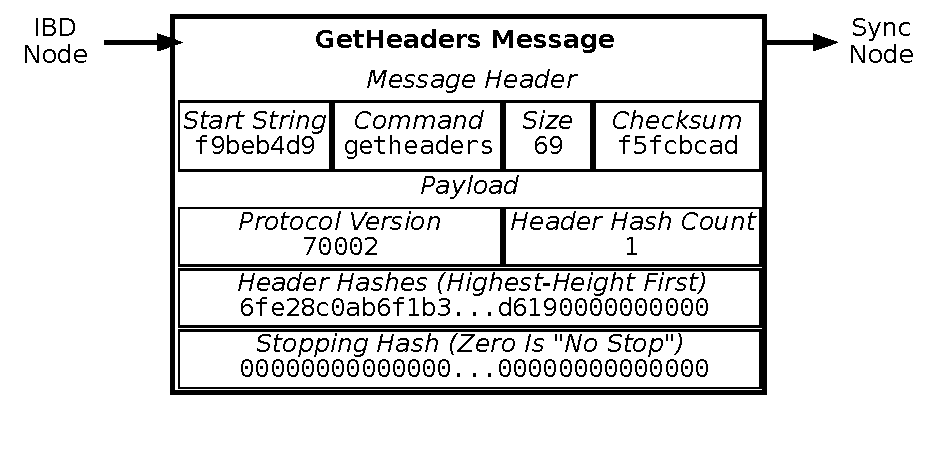
\includegraphics[width=0.7\linewidth]{image/getheaders}
	\caption{مثالی از پیام \texttt{getheaders} در همگام‌سازی اولیهٔ یک گره جدید}
	\label{fig:getheaders}
\end{figure}


گره هم‌گام‌ساز در پاسخ به پیام \texttt{getheaders} در شکل \ref{fig:getheaders} دنبال بلوکی با چکیده مشخص شده می‌گردد و می‌یابد که این بلوک برابر بلوک شمارهٔ صفر (بلوک جنسیس) است. به این ترتیب $۲۰۰۰$ سرایند بلوک را که از بلوک شمارهٔ یک آغاز می‌شوند در قالب پیام \texttt{headers} برای گره درخواست دهنده ارسال می‌کند. قالب این پیام در جدول \ref{table:HeadersMessage} مشخص شده‌ است. شکل \ref{fig:headers} مثالی از پیام بازگردانده شده توسط گره هم‌گام‌ساز است.

\begin{table}[!h]
	\centering
	\caption{
		قسمت‌های پیام \texttt{headers} در شبکه همتا‌به‌همتای بیت‌کوین
		\label{table:HeadersMessage}}
	\begin{tabular}{|c|r|}
		\hline
		\textbf{نام} & {\textbf{توضیحات}} \\
		\hline \hline
		
		\lr{count} & {%
			تعداد سرایند‌های بلوک قرار گرفته در بخش بعدی این پیام. (حداکثر $2000$)
		} \\
		\hline
		
		\lr{headers} & {%
			سرایند‌ بلوک‌ها در این قسمت قرار می‌گیرند.
		} \\
		\hline
	\end{tabular}
\end{table}

\begin{figure}[!h]
	\centering
	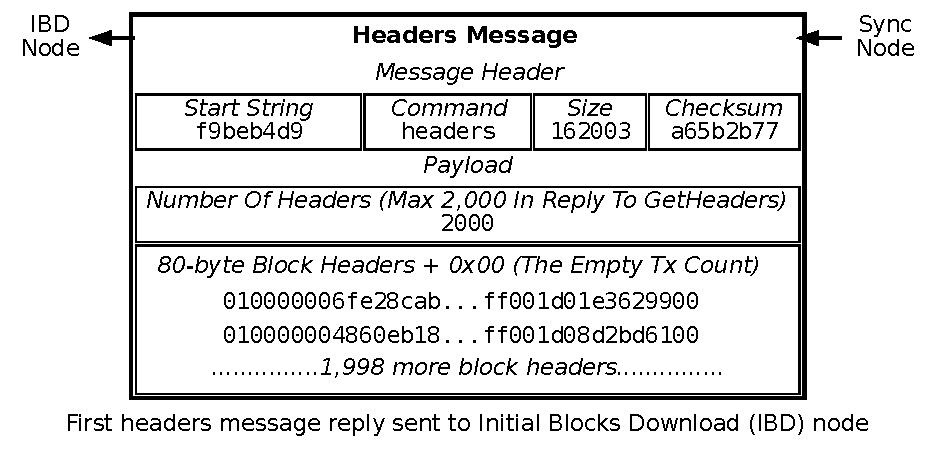
\includegraphics[width=0.7\linewidth]{image/headers}
	\caption{مثالی از پیام \texttt{headers} در همگام‌سازی اولیهٔ یک گره جدید}
	\label{fig:headers}
\end{figure}

وقتی گره سبک پاسخ شکل \ref{fig:headers} را دریافت کرد، فورا صحت آن را بررسی کرده و مجددا پیام  \texttt{getheaders} جدیدی برای گره همگام‌ساز برای گرفته باقیمانده سرایند‌ها ارسال می‌کند. این فرایند تا گرفتن کامل سرایند‌ها ادامه پیدا می‌کند. در زمان نوشتن این پایان‌نامه، حجم تمام سرایند‌های زنجیرهٔ بلوکی ۵۰ مگابایت است. پس از اتمام دانلود سرایند‌های زنجیرهٔ  بلوکی، گره سبک آخرین پیام \texttt{getheaders} را برای چند همتای دیگر ارسال کرده و پاسخ آن‌ها را با پاسخ گره هم‌گام‌ساز ابتدایی مقایسه می‌کند. به این ترتیب مطمئن می‌شود که بهترین سرایند زنجیرهٔ بلوکی را دریافت کرده است. 

\section{انتشار}

زمانی که گره کامل یک بلوک جدید را دریافت می‌کند، پیام \texttt{inv} را برای همهٔ همتا‌هایش (چه گره کامل چه گره سبک) ارسال می‌کند. پیام ارسال شده دارای یک 
%مدخل فهرست \RTLfootnote{Inventory} 
\gls{Inventory}
مربوط به بلوک جدید است. یک مدخل فهرست، شامل یک علامت نوع داده و یک  چکیده داده به عنوان مشخص‌کنندهٔ آن است. داده می‌تواند انواع مختلفی داشته باشد، به عنوان نمونه، علامت تراکنش
\lr{``MSG\_TX''}
و علامت بلوک
\lr{``MSG\_BLOCK''}
است.
به صورت کلی مدخل فهرست به وجود تراکنش‌ها یا بلوک‌هایی برای دانلود اشاره می‌کند. جدول \ref{table:InvMessage} قسمت‌های مختلف پیام \texttt{inv} را شرح می‌دهد. 

\begin{xltabular}{\textwidth}{|c|X|}
	\caption{
		قسمت‌های پیام \texttt{inv} در شبکه همتا‌به‌همتای بیت‌کوین
		\label{table:InvMessage}}\\
	\hline
	\textbf{نام} & {\textbf{توضیحات}} \\
	\hline \hline
	
	\lr{compactSize uint} & {%
		تعداد مدخل‌های فهرست. 
	}\\
	\hline
	
	\lr{inventory} & {%
		یک یا چند مدخل فهرست. حداکثر تعداد آن می‌تواند $50000$ باشد. به عنوان مثال محتوای این قسمت از پیام برای اطلاع‌رسانی بلوک ارتفاع 
		$645747$\LTRfootnote{\url{https://blockchair.com/bitcoin/block/645747}}
		به گره‌های همتا به این صورت است: 
	}\\
	
	&{%
		علامت نوع داده:
		\lr{MSG\_BLOCK}
	}\\
	
	&{%
		مشخص‌کنندهٔ داده (چکیده):
		\lr{\texttt{0x333ab9f10d...0000000000}}
	}\\
	
	\hline
	
\end{xltabular}

گره سبک بعد از دریافت این پیام، یک پیام \texttt{getdata} برای گره کامل می‌فرستد. در این پیام درخواست می‌کند که با توجه به فیلتر بلومی که پیش‌تر در اختیار گره کامل گذاشته بوده، تراکنش‌هایی از بلوک جدید را، که در آن فیلتر صدق می‌کنند برای وی بفرستد. ساختار پیام \texttt{getdata} شبیه \texttt{inv} است. با این تفاوت که علامت نوع داده،‌ اطلاعاتی است که گره ارسال کننده این پیام از گره دریافت‌کننده درخواست می‌کند. 
در این کاربرد، گره سبک علامت \lr{‍‍‍``MSG\_FILTERED\_BLOCK''}  را در کنار چکیده‌ٔ بلوک مورد نظر در پیام قرار می‌دهد و برای گره کامل ارسال می‌کند. به این ترتیب گره کامل تراکنش‌هایی که حداقل یک آدرس آن‌ها در فیلتر بلوم صدق می‌کنند را در کنار اثبات مرکل آن‌ها برای گره سبک ارسال می‌کند.
پاسخ در قالب یک پیام \texttt{merkleblock} که شامل اثبات مرکل وجود تراکنش‌های مرتبط در بلوک است و تعداد صفر یا چند پیام \texttt{tx} را که خود تراکنش‌ها هستند خواهد بود. 
